\documentclass[letterpaper, 10 pt, conference]{ieeeconf}

\IEEEoverridecommandlockouts
\overrideIEEEmargins

\usepackage{fontspec}
\usepackage{xeCJK}
\usepackage{amsmath,amssymb}
\usepackage{booktabs}
\usepackage{graphicx}
\usepackage{hyperref}
\usepackage{xcolor}

\defaultfontfeatures{Ligatures=TeX}
\setCJKmainfont{Microsoft YaHei}
\hypersetup{hidelinks}

\graphicspath{{figures/}}

\title{\LARGE \bf
SE(3)-WAM：面向动态场景操作的世界动作模型
}

\author{Anonymous Authors}

\begin{document}

\maketitle
\thispagestyle{empty}
\pagestyle{empty}

\begin{abstract}
本文给出一个可直接扩展的 ICRA 2027 中文论文骨架。
示例围绕动态场景机器人操作展开，展示章节拆分、公式、表格与参考文献的基本组织方式。
正式投稿前应将正文改为英文，并按照 ICRA 2027 的双匿名与 PDF 合规要求完成检查。
\end{abstract}

\section{Introduction}
\label{sec:introduction}

A moving object can leave its observed position before a robot reaches it.
The same problem arises when a receptacle moves during release or an obstacle
changes the available approach corridor. Dynamic manipulation therefore requires
spatial accuracy at the right time. Faster inference and more responsive
execution reduce observation age \cite{dynamicvla}, while temporal observations
help distinguish motions that look similar in a single image \cite{domino,dynamicwam}.
Together, these demands motivate a practical question:
\emph{what should a robot remember and predict so that its action remains useful
when interaction occurs?}

\begin{figure*}[t]
\centering
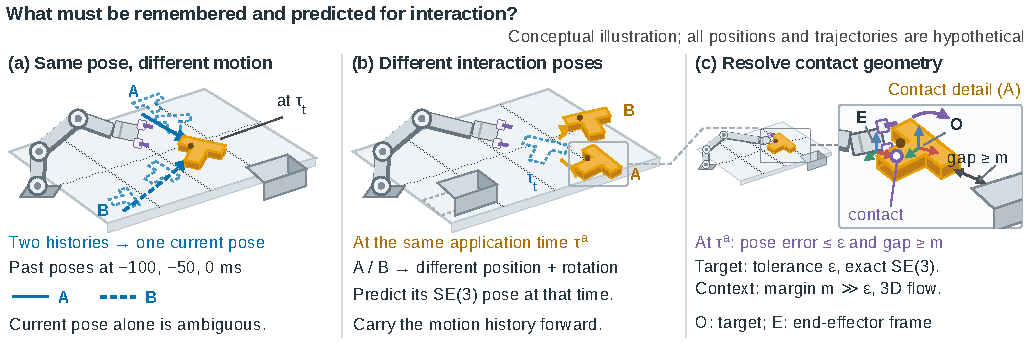
\includegraphics[width=\textwidth]{interaction_timing.pdf}
\caption{What information matters at interaction time?
(a) Two histories meet at the same current target pose.
(b) They lead to different poses at the same future time (solid A, dashed B).
(c) A contact detail for A shows end-effector/target alignment and context clearance.
The same asymmetric target and robot connect the panels. All trajectories
are conceptual illustrations of the research question.}
\label{fig:teaser}
\end{figure*}

The answer depends on the role of information in the task. Target translation
and rotation determine where and how to make contact. A moving occluder or
obstacle matters through its effect on visibility, reachability, or collision.
Static geometry can remain essential even though it has no motion to predict.
This suggests organizing scene evolution by interaction needs: preserve
fine target information when contact requires it, and represent surrounding
changes at sufficient resolution to support the decision. Both a fixed
target/context decomposition and a shared representation with task-dependent
readout can implement this idea. Their relative value is an empirical question.

World--action models provide a framework for learning scene evolution alongside
robot actions \cite{dreamzero,openwam}. However, a future objective changes several
things at once: the supervised variables, the gradients shaping shared features,
and sometimes the computation used before acting. The action may benefit from
auxiliary supervision even when no forecast is generated at deployment
\cite{fastwam}. Conversely, a geometrically accurate forecast may add no useful
information to an already strong state-conditioned policy. Prediction error,
action improvement, and online forecast use must therefore be measured separately.

We organize the \ours Study around three connected questions.
\textbf{Q1} asks how a finite history should encode motion.
\textbf{Q2} asks which future variables, regions, and resolutions support action.
\textbf{Q3} asks how world and action computation should share parameters and
exchange information. Each study matches its own reference; history, future,
and combination studies use distinct recipes. Cross-comparisons revisit
competitive choices before robot-data pretraining.

The completed comparisons give different outcomes across recipes. Structured
GT motion improves the history reference, and a frozen-policy intervention
reveals dependence on its correctness. Visual-history decodability and action
sensitivity do not translate into an overall success-rate advantage.
Among fifteen future-supervision conditions on 1,260 paired scenes, sparse
trajectories give the highest point estimates but no clear overall gain;
dense 2-D displacement decreases success. A twelve-condition combination
screen yields a candidate whose gains over matched controls are concentrated
on phase passage. An adapted DreamVLA system remains stronger under its own
recipe. These results motivate testing how information affects action,
rather than treating added history or future targets as established benefits.

The current evidence supports two contributions:
\begin{itemize}
\item A dynamic-manipulation study protocol that separates task outcomes,
available information, training supervision, and execution conditions.
\item Controlled history and future-supervision studies that distinguish
readable history, action sensitivity, and task benefit, including a frozen-policy
motion-history intervention and fifteen future-supervision conditions.
\end{itemize}
The supplement details the measured configurations and the remaining design,
pretraining, and transfer protocols.

\section{Related Work}
\label{sec:related_work}

\paragraph{Dynamic manipulation.}
Compensating for the time between sensing and acting is a classical problem, from
control with dead time \cite{smith1957} to catching systems that track the target
with Kalman-type filters and plan an interception
\cite{barshalom2001,allen1993,baeuml2010,marturi2019dynamic}; such systems are
precise but engineered for each object and task. Learned policies have recently been
brought to moving scenes \cite{dynamicvla}. PUMA reads historical optical flow
and is supervised with future object features \cite{domino}, and DynamicWAM conditions
a WAM on flow and kinematic descriptors and executes it with real-time chunking
\cite{dynamicwam}. Both infer past motion from image-space cues, whereas \ours takes
the target's metric SE(3) pose history as input and observes only the current RGB-D
frame. Other dynamic policies forecast salient tokens \cite{ahead}, future images
\cite{dbctfp}, compact future codes \cite{foretime}, or 3D scene dynamics
\cite{physmani} and condition their actions on these forecasts at test time. DynaWM
adapts a base VLA's action chunks for dynamic manipulation \cite{dynawm}, and
DynamicManip synthesizes dynamic demonstrations from a static one \cite{dynamicmanip}.
Execution schemes reduce or hide latency by overlapping inference with execution
\cite{dynamicvla,smolvla}, keeping consecutive chunks consistent \cite{rtc,bid}, or
conditioning on the execution time \cite{vlash}. They decide when actions are computed
and applied, not what the policy represents. DOMINO \cite{domino} and PhysMani-Bench
\cite{physmani} provide diverse dynamic-manipulation tasks, but their released default
evaluation pipelines advance the simulation only after a policy has returned its
prediction. \bench advances the scene during inference and charges each method its
measured latency.

\paragraph{Predictive supervision in WAMs.}
World--action models (WAMs) generate future video and actions in one network
\cite{uwm,uva,dreamzero,openwam_alpha}, building on video prediction as a policy
objective \cite{gr1,seer}. Because generating video is costly, recent work changes what
is forecast, such as dynamic regions, depth, and semantic features \cite{dreamvla}, flow
and geometry alongside RGB \cite{dreamwam}, object masks or slots \cite{maskwam,oawam},
or compact latents \cite{flare,wog}, and asks whether the forecast is needed at test
time. Fast-WAM retains most of the benefit of video modeling without test-time
imagination \cite{fastwam}, and PUMA and SG-WAM drop their predictors after training
\cite{domino,sgwam}. \ours keeps this training-only use but forecasts primarily a metric
4D state rather than pixels, features, or latents, so the target's future pose is
supervised explicitly instead of being left implicit.

\paragraph{Object-centric and geometric motion representations.}
Metric 3D inputs make policies more precise and sample-efficient \cite{peract,dp3}.
Motion has been represented by 2D point tracks \cite{atm,track2act,im2flow2act}, 3D
flow \cite{generalflow,flowdreamer,pointworld,physmani}, and object keypoints or SE(3)
trajectories \cite{kpam,spot,objectforesight}, while rigid-body decompositions have long
been used to learn scene dynamics \cite{se3nets,se3posenets}. These works describe the
scene with one kind of representation, such as dense flow or tracks everywhere, or a
pose for each object. Target-centric predictors, including dynamic VLAs with
object-level forecasts, model only the target's future \cite{domino,spot} and leave out
the bodies that block or push it. DOCIR separates the robot, the target, and obstacles,
but uses these distinctions only as input encodings \cite{docir}. \ours assigns
precision by role: a coarse sparse 3D flow describes the whole scene, while the target,
on which contact depends to within millimeters, is additionally described by its SE(3)
history and forecast.

\section{A Controlled World--Action Design Space}
\label{sec:method}

The study varies an encoder $E_\alpha$, a future representation $Z_\beta$, and a
world--action organization $I_\gamma$. Their configuration is
$c=(\alpha,\beta,\gamma)$, with a shared observation and action interface.
Figure~\ref{fig:architecture} separates these design axes from the common
physical-time protocol. The initial reference configuration provides a comparison
base; it is not a final architecture selection.

\begin{figure*}[t]
\centering
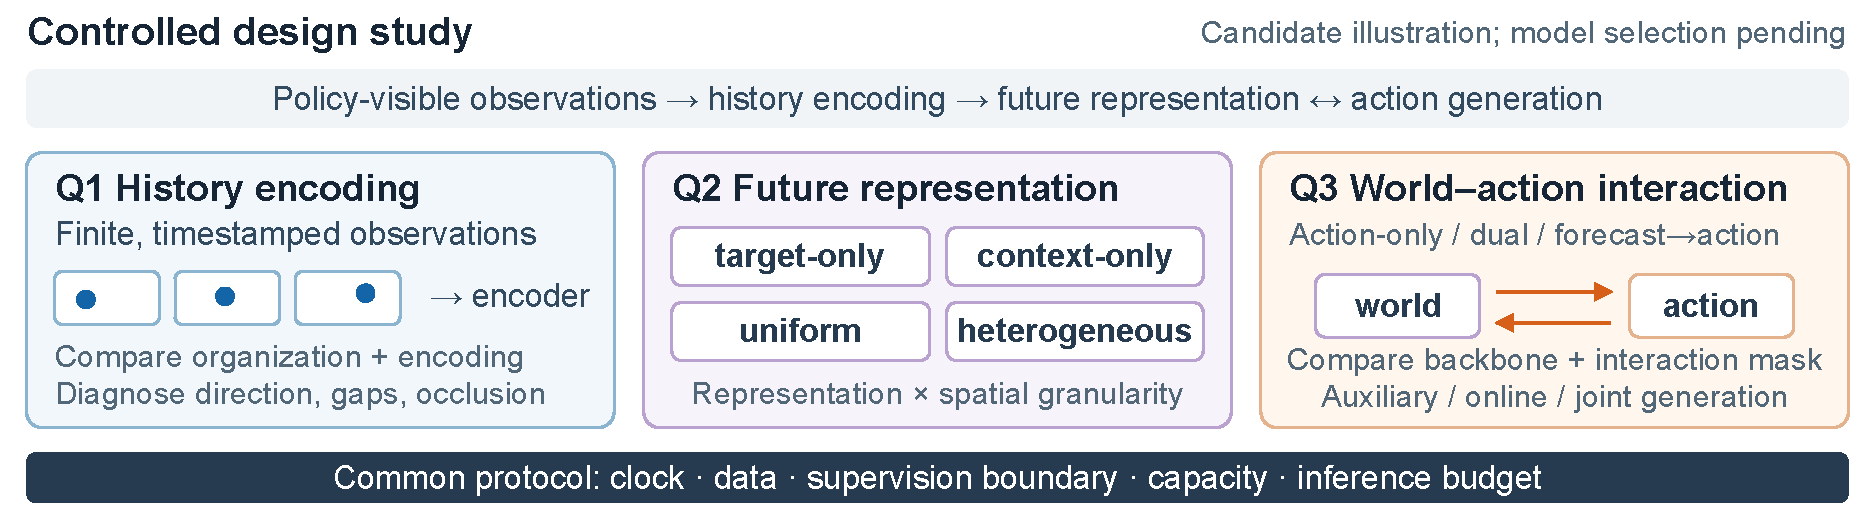
\includegraphics[width=\textwidth]{study_design.pdf}
\caption{The three-axis design study. Q1 changes the encoding of available
history, Q2 changes the future variables and their granularity, and Q3 changes
backbone organization and world--action information flow. Common inputs, physical
times, and budgets define each comparison. Arrows describe conceptual interfaces;
the depicted choices are candidates, not a selected model or measured result.}
\label{fig:architecture}
\end{figure*}

\subsection{Q1: Encoding Finite History}
The encoder maps a finite support of observations to scene and motion tokens:
$\bm X_t=E_\alpha(\mathcal H_t)$. Candidate encodings include RGB history,
time-aware flow, sparse point trajectories, object or scene states, and recurrent
geometric memory. Each specifies coordinate frame, sampling interval, camera
motion, visibility, and early-history validity. Raw displacement without elapsed
time is not a velocity representation. Methods either share the available
history support and token budget or explicitly report the difference. Object
pose and kinematics provided by GT are separate information conditions.
Q1 is evaluated with a stated reference future target and interaction; its
ranking is revisited after Q2 changes what history must support.

An encoding comparison separates access to information from its organization.
One contrast keeps the physical history window fixed while changing the token
representation; another varies the window within the same encoder. They answer
different questions and are not pooled. Flow and trajectories are expressed
relative to declared frames with their true time intervals. Camera-induced
motion must be accounted for or explicitly retained as part of the input.
An early episode with fewer valid observations does not gain synthetic evidence
by repeating its reset frame. A current-object-GT control and a history-object-GT
control hold the remaining robot-state history common, so that their contrast
concerns object information rather than an undeclared change in proprioception.

\subsection{Q2: Future Variables and Granularity}
Given the same available history and execution times, a future predictor forms
\begin{equation}
\hat Z_{\beta,t}=F_\beta(\bm X_t,\{\tau_h^\star\}_{h=0}^{H-1}).
\label{eq:future_interface}
\end{equation}
The target may be rigid pose, trajectory or contact geometry; task-relevant
context may include obstacles, support, moving receptacles, and visibility.
Context is defined by its possible effect on contact, reachability, or collision,
not by a fixed foreground/background split. Static geometry may matter, whereas
unrelated motion need not be predicted.

The comparison distinguishes no future, target-only, context-only, uniform
granularity, and heterogeneous granularity. Representation families such as
RGB or latent state, point trajectories, scene flow, and target \se are
candidates within these roles. A granularity comparison states its region
allocation, spatial and temporal resolution, and decoded-token budget. Changing
both the representation and its budget without a matched control cannot identify
the value of granularity. The action-relevant hypothesis is that preserving
target contact geometry and sufficient contextual constraints may outperform
uniform detail at the same cost; the study also allows the uniform alternative
or auxiliary-only prediction to prevail.

Role and representation are also distinct factors. Comparing target \se with
whole-scene RGB changes both what is described and how it is described. We
therefore record each candidate's target identity source, contextual support,
state variables, spatial allocation, temporal sampling, and prediction budget.
Where the same representation permits it, target-only, context-only, and combined
conditions isolate role coverage. Within a compatible combined representation,
uniform and heterogeneous allocations test granularity while retaining the
same information source and prediction-token allowance. Cross-family comparisons
then report both native prediction error and common action outcomes; a latent
reconstruction loss is not numerically ranked against centimeters of pose error.
These conditional contrasts support a narrower, interpretable conclusion than
a single table in which every row changes role, modality, and cost together.

Temporal resolution is part of granularity. Sampling many future steps at equal
frame intervals can allocate most computation away from the command's execution
window. Each predictor therefore declares the physical horizons it covers and
how the action program queries or pools them. Any extra horizon, adaptive region
selection, or forecast refinement is charged to the same end-to-end budget.
The study can retain a simpler forecast when additional detail is accurate but
does not improve the relevant contact or constraint decision.

For the rigid-target candidate, for example,
\begin{equation}
\hat{\bm T}_h=\Exp(\hat{\bm\xi}_h^\wedge)\hat{\bm T}_t,
\qquad \hat{\bm T}_h\in\se .
\label{eq:se3_prediction}
\end{equation}
This is an output parameterization, not an equivariance claim. Dense displacement
or uncertainty can be added only with its own consumer and evaluation. Predicted
external motion, action-conditioned consequences, and desired task trajectories
are labeled separately. Supplementary Sec.~B gives the inherited \se/flow
candidate mathematics; it does not establish that those heads should survive
model selection.

\subsection{Q3: Backbone Organization and Information Flow}
Q3 compares action-only references, separate world/action systems, prediction
followed by action, and shared or joint world--action organizations. Within a
compatible backbone, interaction masks determine whether action reads future,
future reads action, or both streams interact. Each configuration declares the
visible tokens, gradient paths, generation order, and inference cost; a shared
name does not make two information budgets identical.

Component controls then distinguish auxiliary prediction, online future
conditioning, and joint generation. For the conditional subset these include
\begin{equation}
\begin{aligned}
\text{auxiliary: }&p(\bm a\mid\bm X),\quad q(Z\mid\bm X),\\
\text{online: }&p(\bm a\mid\bm X,\hat Z),\\
\text{joint: }&p(\bm a,Z\mid\bm X).
\end{aligned}
\label{eq:paths}
\end{equation}
Stop-gradient and end-to-end variants address training effects within an
applicable online path; they do not replace the backbone study. A compact
one-way bridge is one such candidate, with zero, swap, noise, and oracle
replacement available when its interface permits a valid intervention. Changing
only the future while fixing perception, robot state, and action-source noise
tests use; a useful effect also requires appropriate action outcomes and safety.

\paragraph{Inference program versus training path.}
A forecast-then-act system makes a world output available before its action
query. A joint generator may instead update action and world variables together;
an action-to-world edge can condition a world output on a proposed action without
feeding a corrected future back into that same action. These programs must be
described by their actual update order, not just by an attention-mask diagram.
The comparison records which intermediate quantities exist when a command is
committed and which are available only during training. In a system without
an independently replaceable forecast, a bridge swap is inapplicable. In a
system that does expose one, a swapped future must preserve the declared
interface and reference condition; replacing arbitrary hidden activations
would test a different perturbation. Backbone allocation, stopping gradients,
and removing an online branch are consequently separate contrasts. Q3 reports
their costs and effects without treating any one intervention as a complete
study of world--action organization.

\paragraph{Selection and cross-comparisons.}
Q1, Q2, and Q3 are compared under stated reference choices, retaining competitive
alternatives for selected cross-checks. Training-only choices and model selection
use the designated development split. The final instance is
\placeholder{history / future / interaction selection}; its description
is filled only after the study and cross-comparisons. More accurate forecasts,
training health, or a fast implementation alone do not select a successful
dynamic policy. Detailed losses, normalization, augmentation, and training
records accompany the actual candidates in Supplementary Secs.~B--E.

\section{Experiments}
\label{sec:experiments}

This section preserves a proposed evaluation design.  Its tables contain pending
fields, not completed runs; budgets and comparisons must be reconciled with the
current Research experiments before execution.  We ask five questions:
\textbf{Q1}, how much do timestamped history and
metric 3-D improve dynamic action? \textbf{Q2}, what does an explicit predicted
future add beyond auxiliary supervision? \textbf{Q3}, is that future physically
accurate and causally used? \textbf{Q4}, how robust is the method to speed, delay,
occlusion, contact, and compute limits? \textbf{Q5}, does the benefit transfer to
native external protocols, static tasks, and a real conveyor?

% Transcribed from results/realtime_c/ (INFER0): ACT/DP native/+150 ms/Paused SR and 5090 p95. Other results pending.
% Highlight reported values per column with \bestcell/\secondcell (SR: highest; p95: lowest); exclude pending cells.
\begin{table}[t]
\centering\footnotesize
\caption{\tablelang{\textbf{Main results.} Task-balanced SR on 1{,}400 held-out \bench scenes: native latency, +150\,ms, and paused physics. Three training seeds for \ours, one per baseline. p95: time-to-action on \cfgGPU{}. Wrist and history denote extra inputs (Sec.~\ref{sec:setup}). Blue/bold and light blue mark the best and second reported values per column; rankings remain provisional while results are pending.}{\textbf{主要结果。}1{,}400 个 \bench 留出场景的任务均衡 SR：原生延迟、+150\,ms 和暂停物理。\ours 训练三个种子，基线各一个。p95：\cfgGPU{} 上的出动作时间。腕部及历史列表示额外输入（第~\ref{sec:setup}~节）。每列已有结果的最佳值为粗体加蓝底，次佳为浅蓝底；结果待齐，排名为暂时性比较。}}
\label{tab:main}
\setlength{\tabcolsep}{0.8pt}
\begin{tabular}{@{}lccccrrrr@{}}
\toprule
 & & \multicolumn{3}{c}{\tablelang{History}{历史}} & \multicolumn{3}{c}{SR (\%) $\uparrow$} & \\
\cmidrule(lr){3-5}\cmidrule(lr){6-8}
\tablelang{Method}{方法} & \tablelang{Wrist}{腕部} & RGB & \tablelang{Flow}{光流} & SE(3) & \tablelang{Native}{原生} & \makecell{+150\\ms} & \tablelang{Paused}{暂停} & \makecell{p95\\(ms)\\$\downarrow$} \\
\midrule
ACT \cite{act} &  &  &  &  & \bestcell{42.0} & \bestcell{24.1} & \bestcell{40.9} & \bestcell{10.7} \\
DP \cite{diffusionpolicy} &  & \cmark &  &  & \secondcell{0.0} & \secondcell{0.0} & \secondcell{33.1} & \secondcell{1701.9} \\
$\pi_{0.5}$ \cite{pi05} &  &  &  &  & \resultplaceholder & \resultplaceholder & \resultplaceholder & \resultplaceholder \\
$\pi_{0.5}$+SE(3) & \resultplaceholder &  &  & \cmark & \resultplaceholder & \resultplaceholder & \resultplaceholder & \resultplaceholder \\
\midrule
DynamicVLA \cite{dynamicvla} &  & \cmark &  &  & \resultplaceholder & \resultplaceholder & \resultplaceholder & \resultplaceholder \\
PUMA \cite{domino} &  &  & \cmark &  & \resultplaceholder & \resultplaceholder & \resultplaceholder & \resultplaceholder \\
\midrule
DreamVLA \cite{dreamvla} &  & \cmark &  &  & \resultplaceholder & \resultplaceholder & \resultplaceholder & \resultplaceholder \\
OpenWAM-$\alpha$ \cite{openwam_alpha} &  &  &  &  & \resultplaceholder & \resultplaceholder & \resultplaceholder & \resultplaceholder \\
\midrule
DynamicWAM \cite{dynamicwam} &  &  & \cmark &  & \resultplaceholder & \resultplaceholder & \resultplaceholder & \resultplaceholder \\
DynamicWAM+SE(3) & \resultplaceholder &  & \cmark & \cmark & \resultplaceholder & \resultplaceholder & \resultplaceholder & \resultplaceholder \\
\midrule
\ours &  &  &  & \cmark & \resultplaceholder & \resultplaceholder & \resultplaceholder & \resultplaceholder \\
\bottomrule
\end{tabular}
\end{table}

\begin{table*}[t]
  \centering
  \caption{Physical forecast quality and causal use.  Forecast metrics use P0
  and exogenous pre-contact windows; intervention deltas are paired within
  exact-current groups so that only the physical summary changes.}
  \label{tab:mechanism_results}
  \scriptsize
  \resizebox{\textwidth}{!}{%
  \begin{tabular}{@{}lcccccccc@{}}
    \toprule
    Model / intervention & Trans. error (cm) $\downarrow$ & Sym.-aware rot. ($^\circ$) $\downarrow$ & EPE3D (cm) $\downarrow$ & Flow--\se{} $\downarrow$ & Core SR (\%) $\uparrow$ & $\Delta\|a\|$ $\uparrow$ & $\Delta$SR (pp) & Interpretation \\
    \midrule
    C1 current-only world & \Pending & \Pending & \Pending & \Pending & -- & -- & -- & observability floor \\
    C9 direct world & \PoseADE & \RotADE & \FlowEPE & \FlowSEConsistency & -- & -- & -- & forecast quality \\
    J-Joint action & \multicolumn{4}{c}{same world/data envelope} & \Pending & 0 (by design) & 0 (by design) & auxiliary supervision \\
    \ours{} P-Detach & \multicolumn{4}{c}{predicted physical summary} & \DBCoreOurs & -- & -- & explicit consumption \\
    \quad swap summary & -- & -- & -- & -- & -- & \SwapActionDelta & \SwapSRDelta & exact-current causal test \\
    \quad zero summary & -- & -- & -- & -- & -- & \Pending & \ZeroSRDelta & information removal \\
    \quad calibrated noise & -- & -- & -- & -- & -- & \Pending & \NoiseSRDelta & sensitivity \\
    \quad oracle summary & 0 & 0 & 0 & 0 & \Pending & \Pending & \Pending & controllability ceiling \\
    \bottomrule
  \end{tabular}%
  }
\end{table*}


\subsection{Setup and Matched Baselines}

\begin{table}[t]
  \centering
  \caption{Matched training and evaluation protocol.}
  \label{tab:implementation}
  \scriptsize
  \begin{tabularx}{\columnwidth}{@{}lX@{}}
    \toprule
    Item & Contract \\
    \midrule
    Observation & 2-view RGB-D, $224^2$; robot/gripper; issued/applied actions; timestamps and validity \\
    Clock & 20 Hz sensing/control; 500 Hz physics; measured capture-to-act delay \\
    Context & C1/C2/C3/C9 views over at most 0.4 s; no repeat padding \\
    World target & $H=8$ at 50--400 ms; target \se, patch 3-D displacement, uncertainty \\
    Action & E7, $H_a=8$; newest-wins continuous execution \\
    Encoder & Frozen DINOv3; depth lift to base-frame XYZ; 4-layer, $d=256$ MIN tier \\
    Optimization & AdamW, $10^{-4}$, cosine decay, 500-step warm-up, effective batch 64 \\
    Evidence & 3 seeds for screening; 5 for headline; 100 paired rollouts/headline cell \\
    \bottomrule
  \end{tabularx}
\end{table}


The proposed matched comparison uses the same demonstrations, frozen DINOv3 features,
history mask, action space, optimizer schedule, parameter envelope, controller,
and paired evaluation manifest.  Its candidate arms are: (1) current-only Action; (2) a
history-aware reactive transformer; (3) a validation-selected constant-position,
velocity, or acceleration retargeter; (4) \emph{J-Joint}, whose future prediction
is auxiliary only; (5) \emph{P-Detach}, the proposed one-way physical interface;
(6) \emph{P-E2E}, which permits action gradients into that interface; and (7)
future-XYZ and future-$\se$ oracles.  Direct regression and action flow matching
would be selected before explicit future information is introduced.  External PUMA,
DynamicVLA, and PhysMani comparisons require native code and scoring.

\subsection{Estimands and Statistical Protocol}

Each design claim is paired with an identifying contrast: history length for
observability, J-Joint versus P-Detach for forecast consumption, exact-current
interventions for causal use, and XYZ versus $\se$ for orientation.  The primary
estimand is the paired Core-SR difference between P-Detach and the strongest
matched history-aware policy.  Secondary outcomes are TC, CT
conditional on success, unsafe contact, and per-task SR.  For an explicit-future
method $P$, history baseline $B$, and future oracle $O$, the oracle-gap fraction is
\begin{equation}
  G_{\mathrm{oracle}}=
  \frac{\operatorname{SR}(P)-\operatorname{SR}(B)}
       {\operatorname{SR}(O)-\operatorname{SR}(B)}.
  \label{eq:oracle_gap}
\end{equation}
The historical protocol proposes a paired bootstrap and five seed-level values
with 100 paired rollouts per seed; these are planned counts, not completed trials.
Wilson intervals
describe individual SRs; a clustered paired bootstrap resamples exact-current
groups within seed for method differences.  Horizon, task, visibility, and motion
factor are declared strata.  Test-OOD, static, external, and real-robot tracks are
opened only after model selection and remain separate estimands.

\subsection{Closed-Loop Manipulation}

Table~\ref{tab:main_results} reserves the primary matched comparison.  Pending
fields are Core SR (\DBCoreOurs\%), TC (\DBCoreTC), CT (\DBCoreCT\ s), matched
history-policy SR (\DBCoreHistory\%), paired difference (\DBCoreDelta\ points,
95\% CI \DBCoreCI), and unsafe-contact rate (\DBCoreUnsafe\%).  The comparison
must separately test the value of history, metric 3-D, and P-Detach versus
J-Joint under the same world targets and action objective.  Per-task and
speed--delay--TTC results are needed to rule out gains confined to one easy cell
or explained by lower action age.

Future oracles test whether headroom exists beyond a strong history policy.
The gap-closed field (\OracleGapClosed\%) remains pending and is interpretable
only if the oracle denominator supports a meaningful comparison.  Neither
P-Detach nor P-E2E is established as superior by this manuscript.

\subsection{Forecast Quality and Causal Use}

The pending world-quality fields are \PoseADE\ cm translation error,
\RotADE$^\circ$ symmetry-aware rotation error, \FlowEPE\ cm 3-D EPE, and
\FlowSEConsistency\ Flow--$\mathrm{SE}(3)$ consistency
(Table~\ref{tab:mechanism_results}).  Error is reported at each physical horizon
and stratified by visibility, speed, acceleration, and rotation.  Pose and dense
flow have proposed complementary roles: target $\se$ for rigid grasp alignment,
and flow for mover awareness and consistency outside the target region.  Those
roles need their own controlled evidence.

Exact-current interventions test causal use of the physical bridge.  Pending
fields record swap action change (\SwapActionDelta), swap SR change
(\SwapSRDelta\ points), and zero/noise SR changes (\ZeroSRDelta/\NoiseSRDelta\
points).  A valid intervention holds the current image, robot state, and
action-source noise fixed while changing only $\bm z$.  The T1-XYZ/SO3 comparison
must test orientation utility with the centroid trajectory held fixed.  Action
sensitivity alone does not show useful foresight: forecast quality, behavior,
safety, and oracle direction must support the same interpretation.

\subsection{Delay Conditions, Systems Profiling, and Transfer}

\begin{table*}[t]
  \centering
  \caption{External validity, static compatibility, real robot, and real-time
  execution. Every external row uses its named native or preregistered protocol;
  no external score is pooled with DB0.}
  \label{tab:external_results}
  \scriptsize
  \begin{tabular}{@{}llrcccc@{}}
    \toprule
    Track & Protocol / primary metric & Trials per model & Reference policy & \ours & Paired $\Delta$ & 95\% CI \\
    \midrule
    DOMINO~\cite{domino} & DOMINO-SA10 SR (\%) & 1,000 & \Pending & \Pending & \Pending & \Pending \\
    DOM~\cite{dynamicvla} & DOM-Dyn4 SR (\%) & 800 & \Pending & \Pending & \Pending & \Pending \\
    PhysMani~\cite{physmani} & Dyn16 normal/high SR (\%) & 640 & \Pending & \Pending & \Pending & \Pending \\
    LIBERO~\cite{libero} & Static40 task-ID SR (\%) & 2,000 & \Pending & \Pending & \Pending & \Pending \\
    Real Franka & Conveyor SR (\%) & 180 & \Pending & \Pending & \Pending & \Pending \\
    \midrule
    Runtime & Inference p50 / p95 (ms) & -- & -- & \LatencyMedian{} / \LatencyTail & -- & -- \\
    Runtime & Action-age p95 / miss rate & -- & -- & \ActionAgeTail{} ms / \DeadlineMiss\% & -- & -- \\
    \bottomrule
  \end{tabular}
\end{table*}


DB0 reports task outcomes at each fixed-delay condition; delay is an ablation axis,
not a score.  A separate batch-one profile reports \LatencyMedian/\LatencyTail\ ms
p50/p95 loop time, \ActionAgeTail\ ms p95 action age, and \DeadlineMiss\% deadline
misses; none is read from the offline dataset.  Table~\ref{tab:external_results}
reserves separate native DOMINO-SA10, DOM-Dyn4, PhysMani-Dyn16, LIBERO-Static40,
and real-conveyor comparisons from the historical plan.  No transfer benefit,
static compatibility, or real-conveyor success is established by these placeholders.

Event traces should distinguish reachability failures, occlusion, and responses
to unannounced impacts.  Their relative frequency and the policy's actual
reactions remain unmeasured here; they cannot yet support a failure taxonomy or
a claim that action-time alignment improves closed-loop control.

\balance
\section{Limitations and Conclusion}
\label{sec:conclusion}

\ours targets single-arm manipulation of task-specified, exogenously moving rigid
objects over short horizons.  It does not model language-conditioned target
selection, long-horizon task planning, multi-object identity, deformables, or
counterfactual contact outcomes under unseen robot actions.  Dense flow after
contact is scored only under matched applied actions, and confidence estimates do
not by themselves constitute a safety guarantee.  The target-centric interface
also depends on sufficient depth quality and visible history; abrupt unobserved
events require re-observation and replanning rather than impossible prediction.

Within this scope, \ours frames dynamic manipulation around when an action takes
effect, combining timestamped metric 3-D history, explicit future
\se/flow/uncertainty, an intervenable one-way interface, and continuous execution.
DB0 asks whether physically correct foresight improves closed-loop behavior beyond
strong history-aware streaming policies under equal information and budget. Paired
results and interventions in Tables~\ref{tab:main_results}--
\ref{tab:external_results} provide the answer, not forecast visualization alone.


\bibliographystyle{IEEEtran}
\bibliography{references}

\end{document}
